\documentclass{article}
    
\usepackage{Haust2017skil}
\usepackage{caption}
\usepackage{subcaption}

\title{Stærðfræðimynstur í tölvunarfræði \\ Skilaverkefni 10}
\author{}

\begin{document}
\maketitle

Skila skal þessu verkefni á vefnum \href{https://gradescope.com/courses/9487}{Gradescope}. Aðgangskóði fyrir námskeiðið er \textbf{9N834D}. 

Gradescope tekur við .pdf skjölum. Frágangur á þeim skiptir máli. Þau skulu vera hreinskrifuð í tölvu. Kerfi eins og \LaTeX, Google Docs og Microsoft Word geta búið til .pdf skjöl. Mikilvægt er að merkja á hvaða blaðsíðu .pdf skjalsins hver lausn kemur fyrir, ekki er hægt að gera ráð fyrir að dæmatímakennarar fari yfir ómerkt dæmi.

Skila má þessum dæmum sem einstaklingar eða \emph{tvö og tvö saman}.

Telji nemandi að mistök hafi verið gerð við yfirferð skal tilkynna slíkt með tölvupósti til dæmatímakennara. Nálgast má lista yfir hvaða dæmatímakennari fór yfir hvaða dæmi á Piazza-vef námskeiðsins.
\section{Kaflar 10.1 og 10.2}

\question Lítum á óstefnt net sem táknar samfélagstengsl, eins og t.d. eftirfarandi net:

\begin{center}
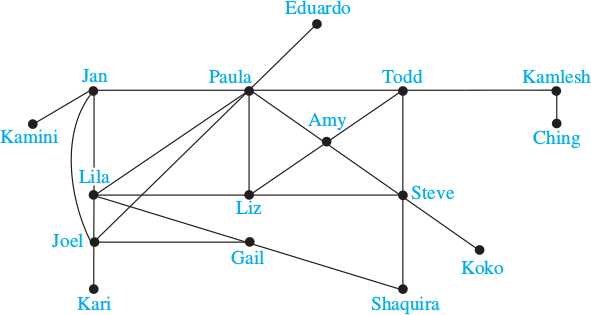
\includegraphics[width=0.5\textwidth]{acquaintanceship}
\end{center}

Gerum ráð fyrir að við séum með net af þessu tagi sem táknar gagnkvæman kunningsskap alls fólks í heiminum. Hvað táknar stig hnúts í slíku neti? Hvað tákna hnútar af stigi 0? Hvað táknar nágrannamengi hnúts? Hvað táknar það að meðalstig hnúta í þessu neti sé 1000?

\paragraph{Í bók:} 10.2.12 í International/Icelandic, 10.2.8 í Global

\newpage

\question Sýnið að einfalt óstefnt net $G$ sem inniheldur að minnsta kosti tvo hnúta hafi að minnsta kosti tvo hnúta af sama stigi.

\paragraph{Í bók:} 10.2.18 í International/Icelandic, 10.2.14 í Global

\paragraph{Ábending:} Við gerum eins og venjulega ráð fyrir að netið sé endanlegt. Hvert er þá hæsta mögulega stig sem hnútur í netinu getur haft?

\question Á eyju nokkurri með ellefu íbúa eru fimm konur og sex karlar sem hyggjast öll ganga í hjónaband. Gert er ráð fyrir að ekkert þeirra viðurkenni áhuga á samkynja hjónabandi eða fjölásta hjónabandi. Konurnar hafa myndað sér skoðun á körlunum, sem eru:

\begin{itemize}
    \item Anna vill ganga í hjónaband með Jason, Larry eða Matt
    \item Barbara vill ganga í hjónaband með Kevin eða Larry
    \item Carol vill ganga í hjónaband með Jason, Nick eða Oscar
    \item Diane vill ganga í hjónaband með Jason, Larry, Nick eða Oscar
    \item Elizabeth vill ganga í hjónaband með Jason eða Matt
\end{itemize}

Karlarnir sætta sig af ótilgreindum ástæðum við hvaða konu sem er til í að umbera þá.
\begin{itemize}
    \item[a)] Setjið möguleg hjónabönd á þessari eyju fram með tvíhlutaneti
    \item[b)] Ákvarðið hjónabönd svo að hver kona fái maka sem er henni þóknanlegur
    \item[c)] Er spyrðingin sem samsvarar útdeilingunni í lið b) fullkomin spyrðing frá mengi kvenna til mengis karla? Er spyrðingin af hámarksstærð?
\end{itemize}

\paragraph{Í bók:} 10.2.28 í International/Icelandic, 10.2.24 í Global

\question 

\textbf{(Ísl)} Látum $G$ vera einfalt óstefnt net. Er mögulegt að eftirfarandi talnarunur séu listar yfir stig hnútanna í $G$? Sé slíkt ekki mögulegt, útskýrið af hverju. Sé það hægt, teiknið netið $G$.

\begin{itemize}
    \item[b)] 6, 5, 4, 3, 2, 1
    \item[e)] 3, 3, 2, 2, 2, 2
\end{itemize}

\paragraph{Í bók:} Hluti af 10.2.42 í Icelandic/International, 5.2.30 í Global

\newpage

\section{Kosningareiknirit}

\question 

\paragraph{(Ísl)} Finnið niðurstöður alþingiskosninganna 2017 í fjölmiðli. Staðfestið auglýsta niðurröðun frambjóðenda í kjördæmasæti í Reykjavík suður með D'Hondt töflu.

\paragraph{(En)} Find the results of the 2017 Icelandic parliamentary elections in the media. Confirm the presented assignment of constitutuent MPs in Reykjavík south using a D'Hondt table.

\section{Kafli 10.3}

\question Teiknið óstefnda netið sem hefur eftirfarandi grennslafylki:

\[
\begin{bmatrix}
1& 3& 2\\
3& 0& 4\\
2& 4& 0\\
\end{bmatrix}
\]

\paragraph{Í bók:} 10.3.16 Í International/Icelandic, 10.3.10 í Global

\end{document}
